\documentclass[11pt]{scrartcl}
\usepackage{graphicx}
\graphicspath{{./}}
\usepackage[sexy]{evan}
\usepackage[normalem]{ulem}
\usepackage{hyperref}
\usepackage{mathtools}
\hypersetup{
    colorlinks=true,
    linkcolor=blue,
    filecolor=magenta,      
    urlcolor=cyan,
    pdftitle={Overleaf Example},
    pdfpagemode=FullScreen,
    }

\renewcommand{\baselinestretch}{1.5}

\addtolength{\oddsidemargin}{-0.4in}
\addtolength{\evensidemargin}{-0.4in}
\addtolength{\textwidth}{0.8in}
% \addtolength{\topmargin}{-0.2in}
% \addtolength{\textheight}{1in} 

\usepackage{pgfplots}
\pgfplotsset{compat=1.15}
\usepackage{mathrsfs}
\usetikzlibrary{arrows}

\begin{document}
	\title{Basic Lessons on Olympiad part One} % Beginner
	\date{\today}
	\author{Azzam L. H.}
	\maketitle
    Dokumen ini terdiri dari materi-materi paling dasar dari olimpiade matematika tingkat SMP-SMA dan disertai dengan latihan soal di bagian akhir dokumen ini. Selamat dan semangat belajar! :D
	\section{Tips-tips}
	\begin{enumerate}
	    \item Latihan yang rajin dan \textbf{konsisten} setiap hari walaupun hanya 30 menit.
	    \item Matematika itu ilmu menulis, catat, coba-coba, dan corat-coret. Anda malas menulis dan hanya mau membaca saja? Buang-buang waktu saja.
	    \item Jangan belajar materi pelajaran matematika sekolah dulu (kecuali yang dibutuhkan di olimpiade), langsung latihan soal olimpiade saja. Kemampuan matematis Anda di pelajaran sekolah akan meningkat sejalan dengan kemampuan matematika olimpiade Anda.
	    \item Kuasailah Bahasa Inggris (terutama Bahasa Inggris Matematika) agar anda bisa mempelajari materi-materi luar negeri dan mengerjakan soal-soal kontes luar Indonesia yang (sayangnya) masih jauh lebih bagus dari materi dan soal-soal di Indonesia.
	    \item Rajin-rajin latihan soal dari \href{https://artofproblemsolving.com/community}{Art of Problem Solving - AOPS} (klik tulisan untuk menuju website).
	    \item Usaha tanpa doa = tidak berkah. Ada tangan tak terlihat yang membantu Anda untuk mengerti semua hal di dunia ini.
	    \item Jangan begadang jika tidak perlu, merusak otak.

	\end{enumerate}
	
	\section{Sebelum Anda Belajar Matematika ...}
	\subsection{Common Math Mistakes}
	\begin{enumerate}
	    \item $\dfrac{n}{0} \neq \infty$ tetapi \textbf{seharusnya} $\dfrac{n}{0} = \text{tak terdefinisi}$ dimana $n \neq 0$.\\
	    Kecuali kalau pakai limit, baru benar, yaitu $\lim_{x \rightarrow 0^+} \dfrac{n}{x} = \infty$ dan $\lim_{x \rightarrow 0^-} \dfrac{n}{x} = -\infty$
	    \item Seharusnya $\dfrac{0}{0} = \textbf{tak tentu}$.
	    \item $\pi$ itu \textbf{dibaca "PI"} bukan dibaca "FI". 
	    \item Kalau $\varphi$ baru dibaca \textbf{"FI"}.
	    \item $\sqrt{x} \ge 0$ dengan $x \ge 0$. Jadi, hasil dari $\sqrt{(-x)^2}=|x|$ jadinya $\sqrt{(-2)^2}=2$.
	\end{enumerate}
	\subsection{Logika Dasar}
	\begin{enumerate}
	    \item $A \land B$ dibaca $A$ dan $B$.
	    \item $A \lor B$ dibaca $A$ atau $B$.
	    \item $A \equiv B$ dibaca $A$ ekuivalen $B$ (untuk logika).
	    \item $\exists x$ dibaca ada $x$ atau terdapat $x$.
	    \item $\forall x$ dibaca untuk semua $x$.
	    \item $A \implies B$ dibaca
	    \begin{enumerate}
	        \item $A$ hanya jika $B$,
	        \item $B$ jika $A$,
	        \item $A$ mengimplikasikan $B$,
	        \item $A$ menyebabkan $B$,
	        \item jika $A$ maka $B$.
	    \end{enumerate}
	    \item $A \Longleftarrow B$ dibaca $A$ jika $B$ (kebalikannya $\implies$).
	    \item $A \iff B$ dibaca $A$ jika dan hanya jika $B$. Definisinya adalah $A \iff B \equiv (A \implies B) \land (A \Longleftarrow B)$.
	\end{enumerate}
	Apa bedanya $A \implies B$ dan $A \iff B$? Kalau $A \implies B$ berarti agar pernyataan benar haruslah $B$ benar, $A$ bisa salah atau benar. Kalau $A \iff B$, agar pernyataan benar, haruslah $A$ dan $B$ sama-sama benar atau sama-sama salah. Contohnya:
	\begin{itemize}
	    \item Jika sekarang hujan, maka saya tidak pergi. (Baik sekarang hujan ataupun tidak hujan, bisa saja saya tidak pergi, jadi tidak pengaruh).
	    \item Klise tapi ya.... : Saya bergerak jika dan hanya jika saya tidak diam :).
	\end{itemize}
	\subsection{Himpunan}
	Hanya review, harusnya sejak SMP sudah paham mengenai himpunan / set hehe.
	
	Misalkan $A$ dan $B$ adalah dua himpunan.
	\begin{enumerate}
	    \item $\phi$ atau $\{\}$ adalah himpunan kosong atau himpunan yang tidak mempunyai elemen.
	    \item Banyak elemen dari $A$ dinotasikan dengan $|A|$ (dibaca "kardinalitas dari $A$") atau $n(A)$ .
	    \item $x \in A$ dibaca $x$ elemen dari $A$.
	    \item $A \subseteq B$ dibaca $A$ subset dari $B$ atau $A$ himpunan bagian dari $B$.
	    \item $A \subset B$ dibaca $A$ adalah proper subset dari $B$. Bedanya dengan $\subseteq$?\\
	    $\subset$ itu mirip $<$ dimana tidak mungkin $A \subset A$, tetapi $\subseteq$ itu mirip $\le$ karena mungkin $A \subseteq A$.
	    \item $A \cup B$ dibaca $A$ union $B$ atau $A$ gabung $B$.
	    \item $A \cap B$ dibaca $A$ intersection $B$ atau $A$ irisan $B$.
	    \item $A^c$ atau $A'$ dibaca $A$ komplemen.
	    \item $|A \cup B| = |A|+|B|-|A \cap B|$.
	\end{enumerate}
	
	\subsection{Himpunan Bilangan-bilangan}
	\begin{figure}[h]
	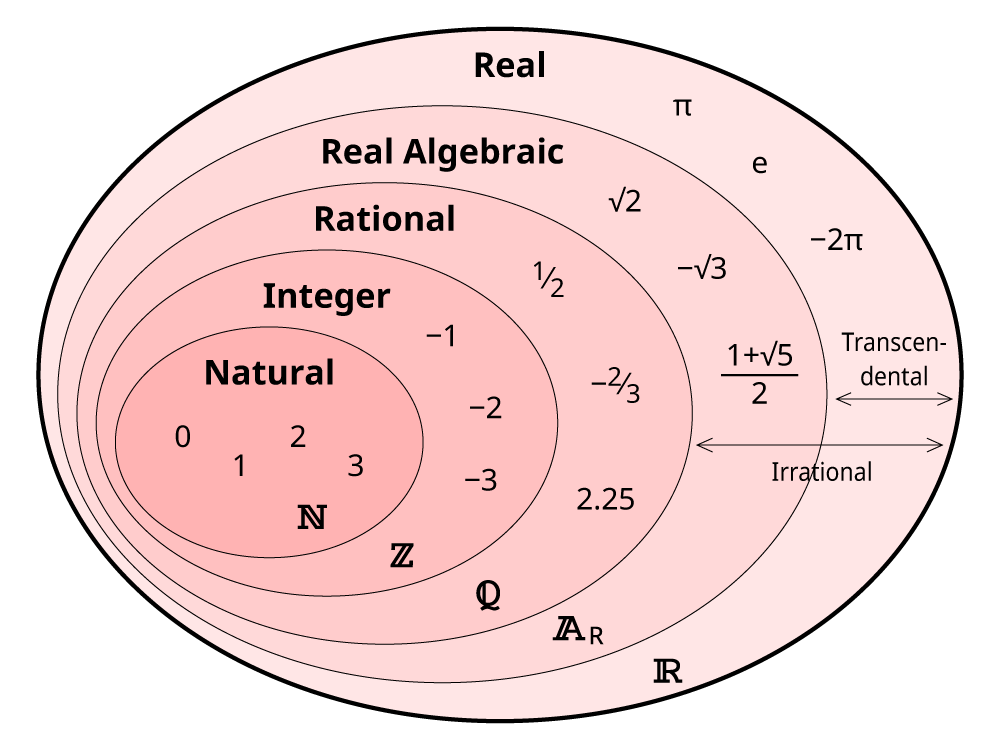
\includegraphics[width=\textwidth/2]{numbers set.png}
	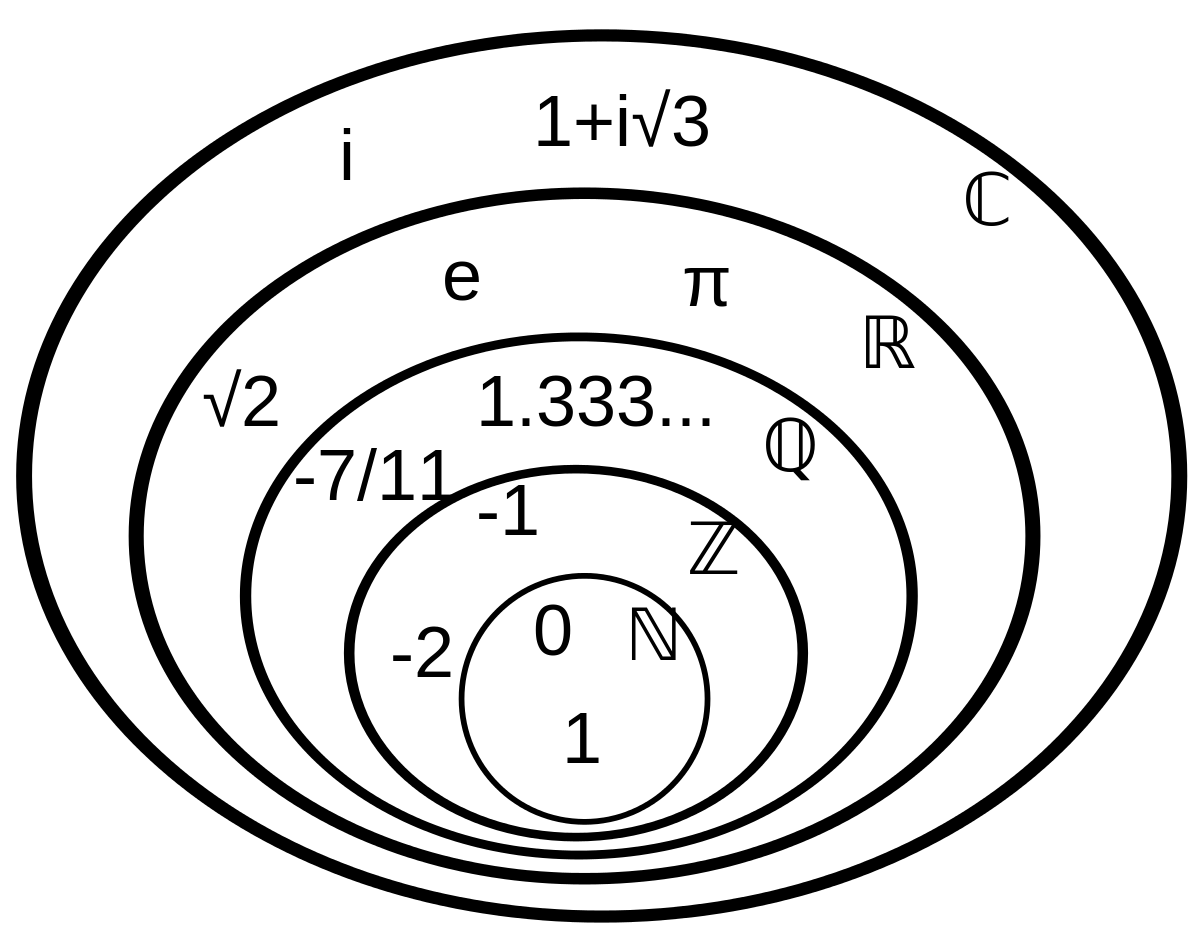
\includegraphics[width=\textwidth/2]{compset.png}
	\caption{dari: https://thinkzone.wlonk.com/Numbers/RealSet\_w1000.png}
	\caption{dan https://en.wikipedia.org/wiki/Number}
	\end{figure}
	
	\begin{enumerate}
	\item $\NN$ adalah himpunan bilangan asli (Natural Numbers) $\{1,2,3,\dots\}$. Di beberapa negara Eropa dan beberapa negara lain, himpunan bilangan asli adalah $\{0,1,2,\dots\}$.
	\item $\ZZ$ adalah himpunan bilangan bulat $\ZZ=\{\dots,-2,-1,0,1,2,\dots\}$.
	\item $\QQ$ adalah himpunan bilangan rasional, dengan definisi $\QQ=\{\dfrac{a}{b}\mid a\in \ZZ, b\in\ZZ^+\}$.
	\item $\RR$ adalah himpunan bilangan real, semua bilangan yang ada di dunia nyata, termasuk bilangan irasional seperti $\sqrt{2}$ dan rasional.
	\item $\CC$ adalah himpunan bilangan kompleks dengan definisi\\ $\CC = \{a+bi \mid a,b \in \RR \text{ dan }i=\sqrt{-1}\}$.
	\item Definisikan pula $\ZZ^+$ sebagai himpunan bialangan bulat positif. Aturan yang sama juga berlaku: $\RR^+, \QQ^+$.
	\end{enumerate}
	

	
	\section{Aljabar}
	\subsection{Pemfaktoran dan Penguraian}
	Pelajaran dari SMP ini mahh. Jangan dihafal secara sengaja, tetapi banyak-banyaklah latihan soal, nanti hafal sendiri :D.
	
	Untuk $x,y,z \in \CC$.
	\begin{enumerate}
	    \item $x^2-y^2 = (x+y)(x-y)$.
	    \item $(x+y)^2 = x^2+2xy+y^2$.
	    \item $(x+y+z)^2 = x^2+y^2+z^2+2xy+2yz+2zx$.
	    \item $(x-y)^2 = x^2-2xy+y^2$.
	    \item $x^3-y^3 = (x-y)(x^2+xy+y^2)$.
	    \item $x^3+y^3 = (x+y)(x^2-xy+y^2)$.
	    \item $(x+y)^3 = x^3+y^3+3xy(x+y) = x^3+3x^2y+3xy^2+y^3$. 
	    \item $(x-y)^3 = x^3-y^3+3xy(x-y) = x^3-3x^2y+3xy^2-y^3$. 
	    \item $x^n-y^n = (x-y)(x^{n-1}+x^{n-2}y+x^{n-3}y^2+\dots+xy^{n-2}+y^{n-1})$ untuk $n \in \NN$.
	    \item $x^n+y^n = (x+y)(x^{n-1}-x^{n-2}y+x^{n-3}y^2-\dots+xy^{n-2}+y^{n-1})$ untuk $n$ adalah bilangan asli \textbf{ganjil}.
	    \item $x^2+y^2+z^2+xy+yz+zx = \frac12(x+y)^2+\frac12(y+z)^2+\frac12(z+x)^2$.
	    \item $x^2+y^2+z^2-xy-yz-zx = \frac12(x-y)^2+\frac12(y-z)^2+\frac12(z-x)^2$.
	    \item $x^3+y^3+z^3-3xyz = (x+y+z)(x^2+y^2+z^2-xy-yz-zx)$.
	    \item $(x+1)(y+1)(z+1)=xyz+xy+yz+zx+x+y+z+1$.
	    \item (Identitas Sophie Germain) $x^4+4y^4=(x^2+2xy+2y^2)(x^2-2xy+2y^2)$.
	    \item (Ekspansi Binomial) $(x+y)^n = {n \choose 0}x^ny^0 + {n \choose 1}x^{n-1}y^1+{n \choose 2}x^{n-2}y^2 + \dots + {n \choose n}x^0y^n$.
	    \item (Fermat Two Square Identity) $(a^2+b^2)(c^2+d^2)=(bc+ad)^2+(bd-ac)^2$ untuk $a,b,c,d \in \RR$.
	\end{enumerate}
	
	\section{Teori Bilangan}
	Pada dasarnya aljabar tetapi di ranah bilangan bulat (atau rasional).
	\subsection{Sifat-sifat Penjumlahan dan Perkalian Dua Bilangan Bulat}
    \begin{enumerate}
        \item Bilangan Ganjil ± Bilangan Ganjil = Bilangan Genap 
        \item Bilangan Ganjil ± Bilangan Genap = Bilangan Ganjil 
        \item Bilangan Genap ± Bilangan Ganjil = Bilangan Ganjil 
        \item Bilangan Genap ± Bilangan Genap = Bilangan Genap 
        \item Bilangan Ganjil $\times$ Bilangan Ganjil = Bilangan Ganjil 
        \item Bilangan Ganjil $\times$ Bilangan Genap = Bilangan Genap 
        \item Bilangan Genap $\times$ Bilangan Ganjil = Bilangan Genap 
        \item Bilangan Genap $\times$ Bilangan Genap = Bilangan Genap
    \end{enumerate}
    Dari sifat-sifat perkalian dua bilangan akan didapat bahwa bilangan genap tidak mungkin membagi 
    bilangan ganjil sedangkan bilangan ganjil mungkin membagi bilangan genap. 
    \subsection{Keterbagian}
    Untuk bilangan bulat $a \neq 0$ serta bilangan bulat $b,c,x$ dan $y$, notasikan $a \mid b$ sebagai $a$ membagi $b$. Lalu, $a$ dan $b$ relatif prima atau $a$ dan $b$ koprima (coprime) jika dan hanya jika $FPB(a,b)=1$.
    \begin{enumerate}
        \item Kita dapat menyatakan semua bilangan bulat $c = pq+r$ untuk suatu bilangan bulat $q$ dimana $0 \le r < q$. Jadi, saat $c$ dibagi $p$, maka hasil baginya adalah $q$ dan sisa baginya adalah $r$.
        \item Terdapat suatu bilangan bulat $x$ dimana $a \mid b \iff b=ax$.
        \item $a \mid a$.
        \item $a \mid 0$.
        \item $1 \mid a$.
        \item $a \mid b \implies a \mid bc$.
        \item Untuk $a,b \neq 0$ maka $ab \mid c \implies a \mid c \text{ dan } b \mid c$.
        \item $a \mid b \text{ dan } b \mid c \implies a \mid c$.
        \item $a \mid b \text{ dan } a \mid c \implies a \mid bx + cy$.
        \item Untuk $x \neq 0$ maka $a \mid b \iff xa \mid xb$.
        \item $a \mid b$ dan $b \neq 0$ maka $|a| \le |b|$.
        \item $a \mid bc$ dan $FPB(a,b)=1$ maka $a\mid c$.
    \end{enumerate}
    \subsection{Uji habis dibagi}
    Trik yang suatu saat dapat membuat hidup anda bahagia wkwkwk. Semua rumus ini dapat dibuktikan dengan aritmatika modular.
    \begin{enumerate}
        \item Bilangan $x$ genap jika dan hanya jika digit terakhir $x$ genap.
        \item $3 \mid x$ jika dan hanya jika jumlah digit-digitnya habis dibagi $3$. Contohnya 2931 habis dibagi 3 karena $2+9+3+1=15$ habis dibagi 3.
        \item $9 \mid x$ jika dan hanya jika jumlah digit-digitnya habis dibagi $9$.
        \item $x$ habis dibagi 5 jika dan hanya jika digit terakhir $x$ adalah $0$ atau $5$.
        \item $x$ habis dibagi 11 jika dan hanya jika jumlah selang-seling (alternate sums) dari digit-digitnya habis dibagi 11. Contoh: 945351 habis dibagi 11 karena $9-4+5-3+5-1=11$ habis dibagi 11. 121 habis dibagi 11 karena $1-2+1=0$ habis dibagi 11.
    \end{enumerate}
    
    \subsection{Aritmatika Modular}
    Untuk suatu bilangan asli $m$ dan bilangan bulat $a,b,c$ dan $d$, notasikan $m\mid a-b \iff a \equiv b \mod m$ (dibaca $a$ kongruen $b$ modulo $m$). Simpelnya $a \equiv b \mod m$ adalah $a$ dibagi $m$ bersisa $b$. Contohnya $5 \equiv 2 \mod 3$. $13 \equiv 3 \mod 5$. $10 \equiv -2 \mod 12$.
    \begin{enumerate}
        \item $a \equiv a \mod m$.
        \item $a \equiv 0 \mod m \iff m\mid a$.
        \item $a \equiv b \mod m \iff b \equiv a \mod m$.
        \item $a \equiv b \mod m \text{ dan } b \equiv c \mod m \implies a \equiv c \mod m$.
        \item Jika $a \equiv b \mod m$ dan $d\mid m$ maka $a \equiv b \mod d$.
        \item Untuk semua bilangan asli $k$, $a \equiv b \mod m \iff a^k \equiv b^k \mod m$.
        \item $a \equiv b \mod m \text{ dan } c \equiv d \mod m \implies a+c \equiv b+d \mod m$.
        \item $a \equiv b \mod m \text{ dan } c \equiv d \mod m \implies ac \equiv bd \mod m$.
        \item $\forall k\in \ZZ^+, (am+b)^k \equiv b^k \mod m$.
        \item Jika $ca \equiv cb \mod m$ dengan $FPB(c,m)=1$, maka $a \equiv b \mod m$.
    \end{enumerate}
    
    Penggunaan sifat nomor 8 dapat dimodifikasi sehingga menjadi konsep \textbf{Chinese Remainder Theorem}.
    
    \section{Kombinatorika}
    
    Notasikan $n!=n \times (n-1) \times (n-2) \times \dots \times 3 \times 2 \times 1$ (dibaca $n$ faktorial) dengan $1!=0!=1$.
    
    \subsection{Kombinasi dan Permutasi}
    Permutasi $k$ unsur dari $n$ unsur adalah (urutan diperhatikan)
    $$_nP_K = P_k^n = \dfrac{n!}{(n-k)!}.$$
    Kombinasi $k$ unsur dari $n$ unsur adalah (urutan tak diperhatikan)
    $${n \choose k}=_nC_K = C_k^n = \dfrac{n!}{k!(n-k)!}.$$
    
    \subsection{Permutasi Siklis}
    $n$ objek ditaruh mengelilingi lingkaran maka banyak cara menyusunnya adalah
    $$P_{siklis} =\dfrac{n!}{n} = (n-1)!$$
    
    \subsection{Stars and Bars}
    Banyaknya solusi bulat non-negatif $(x_1,x_2,\dots,x_k)$ dari sistem persamaan $x_1+x_2+\dots+x_k=n$ adalah
    $${n+k-1 \choose k-1}.$$
    Banyaknya solusi bulat positif $(x_1,x_2,\dots,x_k)$ dari sistem persamaan $x_1+x_2+\dots+x_k=n$ adalah
    $${n-1 \choose k-1}.$$
    
    \section{Geometri}
    Pada dasarnya geometri di olimpiade matematika SMA "hanya" tentang lingkaran dan segitiga , "saja". 
    
    \subsection{Garis, Segmen Garis, Sinar (Bukan Vektor ya...)}
    Perlu ditekankan bahwa \textbf{garis tidak sama dengan ruas garis}. Garis panjangnya tak hingga, sedangkan ruas garis atau segmen garis panjangnya terbatas. Gambar di bawah terdiri dari \textbf{garis AB, segmen garis CD, sinar EF}.
\begin{center}
        \definecolor{ududff}{rgb}{0.30196078431372547,0.30196078431372547,1}
\begin{tikzpicture}[line cap=round,line join=round,>=triangle 45,x=1cm,y=1cm]
\clip(-9,-3) rectangle (5,5);
\draw [line width=2pt,domain=-12.65:12.65] plot(\x,{(--18.806--2.68*\x)/3.84});
\draw [line width=2pt] (-4.47,-0.96)-- (-1.65,1.26);
\draw [line width=2pt,domain=-3.19:12.649999999999997] plot(\x,{(--2.1004--2.44*\x)/2.96});
\begin{scriptsize}
\draw [fill=ududff] (-6.53,0.34) circle (2.5pt);
\draw[color=ududff] (-6.38,0.74) node {$A$};
\draw [fill=ududff] (-2.69,3.02) circle (2.5pt);
\draw[color=ududff] (-2.54,3.42) node {$B$};
\draw [fill=ududff] (-4.47,-0.96) circle (2.5pt);
\draw[color=ududff] (-4.32,-0.56) node {$C$};
\draw [fill=ududff] (-1.65,1.26) circle (2.5pt);
\draw[color=ududff] (-1.5,1.66) node {$D$};
\draw [fill=ududff] (-3.19,-1.92) circle (2.5pt);
\draw[color=ududff] (-3.04,-1.52) node {$E$};
\draw [fill=ududff] (-0.23,0.52) circle (2.5pt);
\draw[color=ududff] (-0.08,0.92) node {$F$};
\end{scriptsize}
\end{tikzpicture}
\end{center}
    
    \subsection{Lingkaran}
    
    \begin{center}
    \definecolor{ffwwqq}{rgb}{1,0.4,0}
\definecolor{uuuuuu}{rgb}{0.26666666666666666,0.26666666666666666,0.26666666666666666}
\definecolor{ffqqtt}{rgb}{1,0,0.2}
\definecolor{ttttff}{rgb}{0.2,0.2,1}
\definecolor{xdxdff}{rgb}{0.49019607843137253,0.49019607843137253,1}
\definecolor{ududff}{rgb}{0.30196078431372547,0.30196078431372547,1}
\begin{tikzpicture}[line cap=round,line join=round,>=triangle 45,x=1cm,y=1cm,scale=1.5]
\clip(-7,-2) rectangle (0,3.5);
\draw [line width=2pt] (-3.71,0.7) circle (2.64cm);
\draw [line width=1.2pt] (-1.07,0.7)-- (-5.351768859108188,2.767412637395495);
\draw [line width=0.8pt,color=ttttff] (-5.351768859108188,2.767412637395495)-- (-3.71,0.7);
\draw [line width=0.8pt,color=ttttff] (-3.71,0.7)-- (-5.909770515623599,-0.7596608094324813);
\draw [line width=1.2pt] (-5.909770515623599,-0.7596608094324813)-- (-1.07,0.7);
\draw [line width=2pt,color=xdxdff] (-5.351768859108188,2.767412637395495)-- (-6.308385428488046,1.1668973816814456);
\draw [line width=2pt,color=xdxdff] (-6.308385428488046,1.1668973816814456)-- (-5.909770515623599,-0.7596608094324813);
\draw [line width=1.2pt] (-5.351768859108188,2.767412637395495)-- (-1.3105942592998239,-0.40111402293088494);
\draw [line width=1.2pt] (-1.3105942592998239,-0.40111402293088494)-- (-5.909770515623599,-0.7596608094324813);
\draw [line width=1.2pt,color=ffqqtt] (-5.351768859108188,2.767412637395495)-- (-5.909770515623599,-0.7596608094324813);
\draw [line width=2pt,color=ffwwqq] (-3.71,0.7)-- (-5.630769687365895,1.0038759139815074);
\begin{scriptsize}
\draw [fill=ududff] (-3.71,0.7) circle (0.5pt);
\draw[color=ududff] (-3.6221931954155986,0.843846768592457) node {$O$};
\draw [fill=ududff] (-1.07,0.7) circle (0.5pt);
\draw[color=ududff] (-0.9803781371406202,0.843846768592457) node {$B$};
\draw [fill=xdxdff] (-5.351768859108188,2.767412637395495) circle (0.5pt);
\draw[color=xdxdff] (-5.476098499468215,2.9526640519523077) node {$C$};
\draw [fill=xdxdff] (-5.909770515623599,-0.7596608094324813) circle (0.5pt);
\draw[color=xdxdff] (-6.0554439069846575,-0.8246680050548971) node {$A$};
\draw [fill=xdxdff] (-6.308385428488046,1.1668973816814456) circle (0.5pt);
\draw[color=xdxdff] (-6.507333324847482,1.2493885538539669) node {$D$};
\draw [fill=xdxdff] (-1.3105942592998239,-0.40111402293088494) circle (0.5pt);
\draw[color=xdxdff] (-1.2237032082975259,-0.25690950568878346) node {$E$};
\draw [fill=uuuuuu] (-5.630769687365895,1.0038759139815074) circle (0.5pt);
\draw[color=uuuuuu] (-5.545619948370188,1.145106380501007) node {$F$};
\end{scriptsize}
\end{tikzpicture}
\end{center}
Misalkan $O$ pusat lingkaran dan $A,B,C,D,E$ adalah sembarang titik seperti gambar.
\begin{enumerate}
    \item $CO=OA$ adalah jari-jari dengan $\angle ACO = \angle OAC$.
    \item Misalkan titik $F$ adalah titik tengah tali busur $CA$, maka $OF \perp CA$ atau $OF$ tegak lurus dengan $CA$, dengan kata lain, $F$ adalah proyeksi titik $O$ ke $CA$
    \item (Sudut keliling-sudut pusat) Untuk$\angle COA = 2\angle CBA$.
    \item (sudut keliling) $\angle CBA = \angle CEA$.
    \item $ABCD$ adalah segiempat tali busur atau segiempat siklis  atau $A,B,C,D$ terletak di lingkaran (seperti pada gambar) jika dan hanya jika $\angle CBA + \angle ADC = 180^\circ$.
\end{enumerate}

\section{Segitiga}

\begin{center}
\definecolor{qqzzqq}{rgb}{0,0.6,0}
\definecolor{yqqqyq}{rgb}{0.5019607843137255,0,0.5019607843137255}
\definecolor{qqttcc}{rgb}{0,0.2,0.8}
\definecolor{uuuuuu}{rgb}{0.26666666666666666,0.26666666666666666,0.26666666666666666}
\definecolor{zzttqq}{rgb}{0.6,0.2,0}
\definecolor{ududff}{rgb}{0.30196078431372547,0.30196078431372547,1}
\begin{tikzpicture}[line cap=round,line join=round,>=triangle 45,x=1cm,y=1cm,scale=2]
\clip(-7.9,-3.2) rectangle (0,3.2);
\fill[line width=2pt,color=zzttqq,fill=zzttqq,fill opacity=0.10000000149011612] (-6.165519534412781,1.8403208695207385) -- (-6.617408952275606,-1.1954490658654202) -- (-0.9745846830654554,-1.1722752495647626) -- cycle;
\fill[line width=2pt,color=zzttqq,fill=zzttqq,fill opacity=0.10000000149011612] (-6.165519534412781,1.8403208695207385) -- (-6.617408952275606,-1.1954490658654202) -- (-0.9745846830654554,-1.1722752495647626) -- cycle;
\draw [line width=2pt,color=zzttqq] (-6.165519534412781,1.8403208695207385)-- (-6.617408952275606,-1.1954490658654202);
\draw [line width=2pt,color=zzttqq] (-6.617408952275606,-1.1954490658654202)-- (-0.9745846830654554,-1.1722752495647626);
\draw [line width=2pt,color=zzttqq] (-0.9745846830654554,-1.1722752495647626)-- (-6.165519534412781,1.8403208695207385);
\draw [line width=1.2pt,domain=-8.957964398642034:-0.18667492884309483] 
\draw [line width=1.2pt,color=qqttcc] (-6.165519534412781,1.8403208695207385)-- (-4.708133684869424,-1.1876080996748404);
\draw [line width=1.2pt,color=yqqqyq] (-6.165519534412781,1.8403208695207385)-- (-6.153060138278336,-1.193542089216561);
\draw [line width=2pt,color=zzttqq] (-6.165519534412781,1.8403208695207385)-- (-6.617408952275606,-1.1954490658654202);
\draw [line width=2pt,color=zzttqq] (-6.617408952275606,-1.1954490658654202)-- (-0.9745846830654554,-1.1722752495647626);
\draw [line width=2pt,color=zzttqq] (-0.9745846830654554,-1.1722752495647626)-- (-6.165519534412781,1.8403208695207385);
\draw [line width=2pt] (-3.8005990144458206,-0.06322724293202202) circle (3.035843290122741cm);
\draw [line width=2pt] (-5.267050752412224,-0.02637740656707221) circle (1.1635162287432892cm);
\draw [line width=1.2pt,color=qqzzqq] (-6.165519534412781,1.8403208695207385)-- (-3.795996817670531,-1.1838621577150916);
\begin{scriptsize}
\draw [fill=ududff] (-6.165519534412781,1.8403208695207385) circle (0.5pt);
\draw[color=ududff] (-6.078617723285315,1.9793637673246847) node {$A$};
\draw [fill=ududff] (-6.617408952275606,-1.1954490658654202) circle (0.5pt);
\draw[color=ududff] (-6.5305071411481395,-1.0564061680614731) node {$B$};
\draw [fill=ududff] (-0.9745846830654554,-1.1722752495647626) circle (0.5pt);
\draw[color=ududff] (-0.8876828719379902,-1.0332323517608155) node {$C$};
\draw [fill=uuuuuu] (-6.153060138278336,-1.193542089216561) circle (0.5pt);
\draw[color=uuuuuu] (-6.182899896638275,-1.2765574229177212) node {$D$};
\draw [fill=uuuuuu] (-4.708133684869424,-1.1876080996748404) circle (0.5pt);
\draw[color=uuuuuu] (-4.6186672963438795,-1.0448192599111443) node {$E$};
\draw [fill=uuuuuu] (-3.795996817670531,-1.1838621577150916) circle (0.5pt);
\draw[color=uuuuuu] (-3.703301552467901,-1.0448192599111443) node {$M$};
\draw[color=black] (-5.841086106203574,2.5934698992921135) node {$L1$};
\draw [fill=uuuuuu] (-3.800599014445821,-0.06322724293202069) circle (0.5pt);
\draw[color=uuuuuu] (-3.5758455628142833,-0.0831058834338501) node {$O$};
\draw [fill=uuuuuu] (-5.267050752412224,-0.02637740656707221) circle (0.5pt);
\draw[color=uuuuuu] (-5.174838887559664,0.11387155512174028) node {$I$};
\draw[color=black] (-5.87584683065456,0.8554336767427865) node {$L2$};
\draw [fill=uuuuuu] (-6.156315140862202,-0.40094896004539987) circle (0.5pt);
\draw[color=uuuuuu] (-6.067030815134986,-0.25690950568878285) node {$H$};
\end{scriptsize}
\end{tikzpicture}
\end{center}
Pada segitiga $ABC$,
\begin{enumerate}
    \item Berlaku \textbf{ketaksamaan segitiga} yaitu $AB+BC>CA$, $BC+CA>AB$, dan $CA+AB>BC$. Selain itu juga berlaku $|AB-BC|<CA$, $|BC-CA|<AB$, dan $|CA-AB|<BC$.
    \item Garis bagi $AE$ yaitu garis yang membagi dua sudut $A$ sama besar sehingga $\angle BAE = \angle EAC$. Berlaku \textbf{Teorema Garis Bagi}, yaitu $\dfrac{AB}{AC}=\dfrac{BE}{CE}$.
    \item Garis berat $AM$ dengan $M$ adalah titik tengah $BC$.
    \item Garis tinggi $AD$ adalah garis yang tegak lurus dengan $BC$. $D$ biasa disebut dengan proyeksi $A$ ke $BC$.
    \item Garis $OM$ adalah salah satu garis sumbu segitiga $ABC$, yaitu garis yang melewati titik tengah sisi segitiga dan tegak lurus dengan sisi itu.
    \item Pertemuan atau perpotongan ketiga garis tinggi segitiga $ABC$ adalah titik tinggi, dalam gambar ini adalah $H$ (orthocenter).
    \item Pertemuan atau perpotongan ketiga garis bagi segitiga $ABC$ adalah titik bagi atau titik pusat lingkaran dalam (incircle $L2$) segitiga $ABC$ dalam gambar ini adalah $I$ (incenter).
    \item Pertemuan atau perpotongan ketiga garis berat segitiga $ABC$ adalah titik berat (centroid).
    \item Pertemuan atau perpotongan ketiga garis sumbu segitiga $ABC$ adalah titik pusat lingkaran luar (circumcircle $L1$) segitiga $ABC$ yang dalam gambar ini adalah $O$ (circumcenter).
\end{enumerate}

\subsection{Kesebangunan Segitiga}
\begin{center}
\definecolor{xdxdff}{rgb}{0.49019607843137253,0.49019607843137253,1}
\definecolor{ttttff}{rgb}{0.2,0.2,1}
\definecolor{qqzzff}{rgb}{0,0.6,1}
\definecolor{ududff}{rgb}{0.30196078431372547,0.30196078431372547,1}
\begin{tikzpicture}[line cap=round,line join=round,>=triangle 45,x=1cm,y=1cm]
\clip(-6.5,0.5) rectangle (0.5,4);
\fill[line width=2pt,color=qqzzff,fill=qqzzff,fill opacity=0.1] (-5.933781371406205,1.3073230946056116) -- (-5.37760978019042,2.72092588894573) -- (-3.76702954729471,1.3420838190565978) -- cycle;
\fill[line width=0.8pt,color=xdxdff,fill=xdxdff,fill opacity=0.1] (-3.1992710479285953,0.9944765745467326) -- (-2.283905304052617,3.2307498475601983) -- (0.299975213470717,1.0524111152983768) -- cycle;
\draw [line width=2pt,color=qqzzff] (-5.933781371406205,1.3073230946056116)-- (-5.37760978019042,2.72092588894573);
\draw [line width=2pt,color=qqzzff] (-5.37760978019042,2.72092588894573)-- (-3.76702954729471,1.3420838190565978);
\draw [line width=2pt,color=qqzzff] (-3.76702954729471,1.3420838190565978)-- (-5.933781371406205,1.3073230946056116);
\draw [line width=0.8pt,color=xdxdff] (-3.1992710479285953,0.9944765745467326)-- (-2.283905304052617,3.2307498475601983);
\draw [line width=0.8pt,color=xdxdff] (-2.283905304052617,3.2307498475601983)-- (0.299975213470717,1.0524111152983768);
\draw [line width=0.8pt,color=xdxdff] (0.299975213470717,1.0524111152983768)-- (-3.1992710479285953,0.9944765745467326);
\begin{scriptsize}
\draw [fill=ududff] (-5.933781371406205,1.3073230946056116) circle (0.5pt);
\draw[color=ududff] (-5.846879560278738,1.4463659924095578) node {$A$};
\draw [fill=ududff] (-5.37760978019042,2.72092588894573) circle (0.5pt);
\draw[color=ududff] (-5.290707969062953,2.859968786749677) node {$B$};
\draw [fill=ududff] (-3.76702954729471,1.3420838190565978) circle (0.5pt);
\draw[color=ududff] (-3.6801277361672433,1.4811267168605442) node {$C$};
\draw [fill=ududff] (-3.1992710479285953,0.9944765745467326) circle (0.5pt);
\draw[color=ududff] (-3.1123692368011295,1.133519472350679) node {$D$};
\draw [fill=ududff] (-2.283905304052617,3.2307498475601983) circle (0.5pt);
\draw[color=ududff] (-2.1970034929251505,3.3697927453641463) node {$E$};
\draw [fill=ttttff] (0.299975213470717,1.0524111152983768) circle (0.5pt);
\draw[color=ttttff] (0.38687702459818324,1.191454013102323) node {$F$};
\end{scriptsize}
\end{tikzpicture}
\end{center}

Segitiga $ABC$ dan $DEF$ sebangun atau $ABC \sim DEF$ jika dan hanya jika minimal salah satu syarat ini terpenuhi:
\begin{enumerate}
    \item $\angle ABC = \angle DEF$ dan $\angle BAC = \angle EDF$.
    \item $\dfrac{AB}{DE} = \dfrac{BC}{EF} = \dfrac{CA}{FD}$.
    \item $\dfrac{AB}{DE} = \dfrac{BC}{EF}$ dan $\angle ABC = \angle DEF$ (sudut yang diapit dua sisi yang diperbandingkan nilainya sama)
\end{enumerate}

\subsection{Kekongruenan Segitiga}
\begin{center}
\definecolor{xdxdff}{rgb}{0.49019607843137253,0.49019607843137253,1}
\definecolor{ttttff}{rgb}{0.2,0.2,1}
\definecolor{qqzzff}{rgb}{0,0.6,1}
\definecolor{ududff}{rgb}{0.30196078431372547,0.30196078431372547,1}
\begin{tikzpicture}[line cap=round,line join=round,>=triangle 45,x=1cm,y=1cm]
\clip(-8,0.5) rectangle (0.5,4);
\fill[line width=2pt,color=qqzzff,fill=qqzzff,fill opacity=0.1] (-7.671817593955533,1.110345656050021) -- (-6.756451850079554,3.3582058372138173) -- (-4.184158240706549,1.1914540131023228) -- cycle;
\fill[line width=0.8pt,color=xdxdff,fill=xdxdff,fill opacity=0.1] (-3.8828986287979985,1.191454013102323) -- (-2.9675328849220186,3.4277272861157897) -- (-0.38365236739868475,1.2493885538539673) -- cycle;
\draw [line width=2pt,color=qqzzff] (-7.671817593955533,1.110345656050021)-- (-6.756451850079554,3.3582058372138173);
\draw [line width=2pt,color=qqzzff] (-6.756451850079554,3.3582058372138173)-- (-4.184158240706549,1.1914540131023228);
\draw [line width=2pt,color=qqzzff] (-4.184158240706549,1.1914540131023228)-- (-7.671817593955533,1.110345656050021);
\draw [line width=0.8pt,color=xdxdff] (-3.8828986287979985,1.191454013102323)-- (-2.9675328849220186,3.4277272861157897);
\draw [line width=0.8pt,color=xdxdff] (-2.9675328849220186,3.4277272861157897)-- (-0.38365236739868475,1.2493885538539673);
\draw [line width=0.8pt,color=xdxdff] (-0.38365236739868475,1.2493885538539673)-- (-3.8828986287979985,1.191454013102323);
\begin{scriptsize}
\draw [fill=ududff] (-7.671817593955533,1.110345656050021) circle (0.5pt);
\draw[color=ududff] (-7.584915782828065,1.2493885538539673) node {$A$};
\draw [fill=ududff] (-6.756451850079554,3.3582058372138173) circle (0.5pt);
\draw[color=ududff] (-6.669550038952086,3.4972487350177635) node {$B$};
\draw [fill=ududff] (-4.184158240706549,1.1914540131023228) circle (0.5pt);
\draw[color=ududff] (-4.097256429579081,1.3304969109062692) node {$C$};
\draw [fill=ududff] (-3.8828986287979985,1.191454013102323) circle (0.5pt);
\draw[color=ududff] (-3.7959968176705314,1.3304969109062692) node {$D$};
\draw [fill=ududff] (-2.9675328849220186,3.4277272861157897) circle (0.5pt);
\draw[color=ududff] (-2.8806310737945524,3.5667701839197368) node {$E$};
\draw [fill=ttttff] (-0.38365236739868475,1.2493885538539673) circle (0.5pt);
\draw[color=ttttff] (-0.29675055627121893,1.3884314516579135) node {$F$};
\end{scriptsize}
\end{tikzpicture}
\end{center}
Sedangkan $ABC$ dan $DEF$ dikatakan kongruen atau $\triangle ABC \cong \triangle DEF$ jika dan hanya jika $AB=DE, BC=EF, CA=FD$ atau dengan kata lain kedua segitiga tersebut sebangun dan ada salah satu sisi dari kedua segitiga tersebut yang panjangnya sama. Simpelnya kongruen = sama persis.

\subsection{Trigonometri}
Banyak sih rumusnya, tapi yang paling sering dipake di olim:
\begin{enumerate}
    \item $\sin (-x) = -\sin x$.
    \item $\cos (-x) = \cos x$.
    \item $\tan(-x) = -\tan x$.
    \item $\sin^2 x + \cos^2 x = 1$.
    \item $\sin(90^\circ-x)=\sin(90^\circ+x)=\cos x$.
    \item $\sin(a \pm b) = \sin a \cos b \pm \cos a \sin b$.
    \item $\sin 2x = 2\sin x \cos x$.
    \item $\cos(a \pm b) = \cos a \cos b \mp \sin a \sin b$.
    \item $\cos 2x = \cos^2 x - \sin^2 x = 2\cos^2 x -1 = 1-2\sin^2 x$.
    \item $\tan(a \pm b) = \dfrac{\tan a \pm \tan b}{1 \mp \tan a \tan b}$.
\end{enumerate}
Cara menghafal yang gampang bisa make "metode sumbu" (ask me on training to knows more)
\section{Latihan Soal}
\subsection{Aljabar}
\begin{enumerate}
    \item Jika $x=2021^3-2019^3$, maka nilai $\sqrt{\dfrac{x-2}{6}}$ adalah \dots
    \item  dari $\sqrt{5050^2-4950^2}$ adalah \dots

    \item (OSP 2008) Jika $0 < b < a$ dan $a^2+b^2=6ab$, maka nilai $\dfrac{a+b}{a-b}=\dots$
    
    \item Jika $x > 0$ dan $x + \dfrac{1}{x} =  5$, maka nilai $x^3+\dfrac{1}{x^3}$ adalah \dots
    
    \item (OSK 2017) Diketahui $x-y=10$ dan $xy=10$. Nilai $x^4+y^4$ adalah \dots
    
    \item Jika $a+b+c=0$, buktikan bahwa $a^3+b^3+c^3=3abc$.

    \item (AIME 1987)
    Tentukan nilai sederhana dari $\dfrac{(10^4+324)(22^4+324)(34^4+324)(46^4+324)(58^4+324)}{(4^4+324)(16^4+324)(28^4+324)(40^4+324)(52^4+324)}$
\end{enumerate}


\subsection{Teori Bilangan}
\begin{enumerate}
    \item (OSN SMP 2003) Buktikan bahwa $(n-1)n(n^3+1)$ selalu habis dibagi 6 untuk semua bilangan asli $n$.
    
    \item Carilah semua bilangan bulat $n$ sehingga $\dfrac{2n+6}{n-1}$ adalah bilangan bulat.
    
    \item (OSK 2002) Bilangan asli $n$ terbesar sehingga $8^n \mid 44^{44}$ adalah \dots
    
    \item Berapa banyak pasangan bilangan bulat positif $(a,b)$ yang memenuhi $\dfrac{1}{a}+\dfrac{1}{b}=\dfrac{1}{6}$.
    
    \item Jika $a$ dan $b$ adalah bilangan bulat sedemikian sehingga $a^2-b^2=2017$, maka nilai dari $a^2+b^2$ adalah \dots
    
    \item (AIME 1986) Tentukan bilangan asli $n$ terbesar sehingga $n+10 \mid n^3+100$.
    
    \item (OSK 2010) Nilai $n$ terkecil sehingga $\underbrace{20102010\dots2010}_\text{$n$ buah 2010}$ habis dibagi 99 adalah \dots
    
    \item Jika dihitung maka didapat $17! = 3a56874280b6000$. Tentukan nilai digit $a$ dan $b$.
    
    \item Tentukan digit satuan dari $7^{7^7}$.
    
    \item Jika $S=1!+2!+3!+\dots+2021!$, tentukan sisa $S$ saat dibagi 6.
    
    \item (OSK 2009) Sisa saat $10^{999999999}$ saat dibagi oleh 7 adalah \dots
    \item (OSK 2011) Bilangan asli terkecil $n>2011$ yang bersisa 1 jika dibagi $2,3,4,5,6,7,8,9,10$ adalah \dots.
\end{enumerate}

\subsection{Kombinatorika}
\begin{enumerate}
    \item Misalkan terdapat 3 buah celana dan 4 buah baju. Permasalahannya adalah ada berapa banyak cara 
seseorang memilih celana dan baju yang akan dipakai ?

    \item Berapa banyak cara menyusun huruf-huruf R, A, J, I, N jika 
\begin{enumerate}
    \item huruf pertama dimulai dari huruf hidup (vokal) 
    \item huruf pertama dimulai dari huruf mati (konsonan) 
\end{enumerate}

    \item Sembilan orang siswa akan duduk pada 5 kursi sejajar. Ada berapa cara susunan mereka ? 
    
    \item Denny akan membentuk bilangan genap 3 angka yang angka-angkanya diambil dari 2, 3, 4, 5, 6, 7, 8. 
Berapa banyak bilangan yang dapat dibentuk jika : 
    \begin{enumerate}
        \item angka-angkanya boleh berulang 
\item angka-angkanya tidak boleh berulang
    \end{enumerate}
    
    \item (OSK 2003) Ada berapa banyak bilangan 4-angka (digit) yang semua angkanya genap dan bukan 
merupakan kelipatan 2003 ?
    \item  Carilah banyaknya menempatkan 3 benteng (rooks) pada papan catur $5 \times 5$ sehingga
tidak ada dua catur yang dalam posisi dapat saling menyerang.

    \item Sekumpulan orang duduk mengelilingi sebuah meja bundar. Diketahui ada 7 wanita
dimana di sebelah kanan setiap wanita tersebut adalah wanita dan ada 12 wanita yang di
sebelah kanan setiap wanita tersebut adalah pria. Diketahui pula bahwa 3 dari 4 pria di
sebelah kanannya adalah wanita. Berapa orang yang duduk mengelilingi meja tersebut?

    \item Carilah banyaknya kuadrupel terurut bilangan ganjil positif $(x_1, x_2, x_3, x_4)$ yang memenuhi
$x_1 + x_2 + x_3 + x_4 = 98$.

    \item Perhatikan gambar berikut.\\
    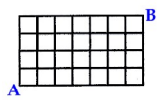
\includegraphics[scale=1.2]{kombin.PNG}
    Jika seseorang akan berjalan dari titik A ke titik B. Ada berapa banyak cara jalan terpendek 
yang dapat dipilihnya ?
    
    \item (OSP 2003) Empat pasang suami istri menonton pagelaran orkestra. Tempat duduk mereka harus 
dipisah antara kelompok suami dan kelompok istri. Untuk masing-masing kelompok disediakan 4
buah tempat duduk bersebelahan dalam satu barisan. Ada berapa banyak cara memberikan 
tempat duduk kepada mereka ?

    \item (OSK 2010) Banyaknya himpunan $X$ yang memenuhi 
$$\{1,2,\dots,1000\} \subseteq X \subseteq \{1,2,\dots,2010\}.$$

    \item (OSP 2010) Bilangan enam digit $abcdef$ dengan $a > b > c \ge d > e > f$ ada sebanyak \dots
    
    \item (OSK 2017)
	Sebuah hotel mempunyai kamar bernomor 000 sampai dengan 999. Hotel tersebut menerapkan
aturan aneh sebagai berikut: jika suatu kamar berisi tamu, dan sembarang dua digit nomor kamar
tersebut dipertukarkan tempatnya, maka diperoleh nomor kamar yang sama atau nomor kamar
yang tidak berisi tamu. Maksimal banyaknya kamar yang berisi tamu adalah \dots
\end{enumerate}

\subsection{Geometri}
\begin{enumerate}
    \item Pada segiempat $WXYZ$ dengan diagonal yang saling tegak lurus diketahui bahwa $\angle WZX = 30^\circ, \angle XWY = 40^\circ,$ and $\angle WYZ = 50^\circ$. Hitunglah besar $\angle X$ dan $\angle Z$.
    
    \item
		Garis berat $AD$ pada segitiga $ABC$ memotong garis berat $CF$ di titik $P$, serta perpanjangan $BP$ memotong $AC$ di $E$. Jika diketahui segitiga $ABC$ lancip dan $AB=6$, maka panjang $DE$ adalah \dots
		
	\item (OSK 2013) Diberikan segitiga lancip $ABC$ dengan $O$ sebagai pusat lingkaran luarnya. Misalkan $M$ dan $N$
berturut - turut pertengahan $OA$ dan $BC$. Jika $\angle ABC = 4\angle OMN$ dan $\angle ACB = 6\angle OMN$,
maka besarnya $\angle OMN$ sama dengan \dots

    \item (\textbf{Soal Legend: OSK 2011,2012,2013,2018}) Diberikan segitiga $ABC$ dan lingkaran $\Gamma$ yang berdiameter $AB$ . Lingkaran $\Gamma$ memotong sisi $AC$ dan $BC$
berturut-turut di titik $D$ dan $E$. Jika $AD = \frac13 AC, BE =\frac14 BC$ dan $AB = 30$, maka luas segitiga $ABC$ adalah \dots
		
	\item
		Diberikan segitiga $ABC$ dengan $D$ titik tengah $AC$, $E$ titik tengah $BD$, dan $H$ merupakan pencerminan $A$ terhadap $E$. Jika $F$ merupakan perpotongan antara $AH$ dengan $BC$, maka nilai $\dfrac{AF}{FH}$ sama dengan \dots
		
	\item 	
		 Pada gambar di bawah, diketahui titik A $\ne$ B pada lingkaran berdiameter $MN$ dan berpusat di $C$. $P$ adalah titik pada segmen $CN$ dimana $\angle CAP = \angle CBP = 10 ^\circ$. Jika $\angle ACM = 40^\circ$, maka $\angle BCN = \dots^\circ$
		 
		 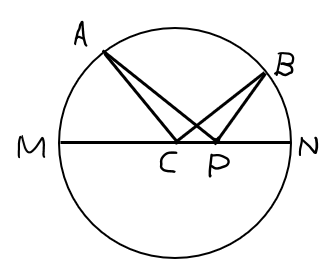
\includegraphics[scale=0.7]{pemanasan post test geom}
		 
	\item
		Diberikan sebuah segitiga dengan panjang sisi $BC = 20$, $CA = 24$, dan $AB=12$. Titik $D$ pada segmen $BC$ dengan $BD = 5$. Lingkaran luar dari segitiga $ABD$ memotong $CA$ di $E$. Hitunglah nilai $2 \times DE$.
		
	\item Jika $A+B=45^\circ$ dan $\cos A\sin B=\frac{\sqrt{2}}{6}$, maka $\cos(B-A)=\dots$
	
	\item Nilai dari $\cos \dfrac{\pi}{7}\cdot \cos \dfrac{2\pi}{7} \cdot \cos \dfrac{4\pi}{7}$ adalah \dots
	
	\item Pada segitiga $ABC$, buktikan bahwa $\tan A + \tan B + \tan C = \tan A \tan B \tan C$.
	
	\item Tentukan nilai eksak dari $\tan 1^\circ \cdot \tan 2^\circ \cdot \tan 3^\circ \cdot \ldots \cdot \tan 89^\circ$.
	
	\item (OSK 2005) Nilai dari $\sin^8 75^\circ - \cos^8 75^\circ$ adalah \dots
\end{enumerate}
\section{Referensi}
\begin{enumerate}
    \item Hermanto, Eddy. 2011. Diktat Pembinaan Olimpiade Matematika Dasar.
\end{enumerate}
\end{document}


